\begin{figure*}[t]
  \centering
  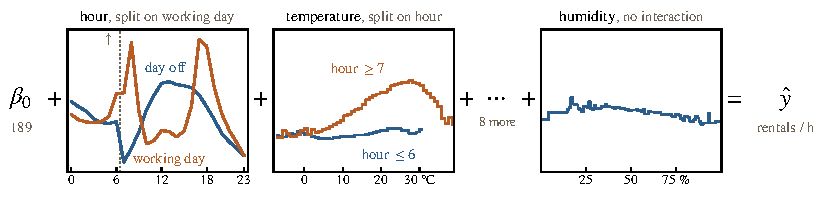
\includegraphics[width=\textwidth]{images/concept.pdf}
  \caption{A CALM fitted on the Bike Sharing dataset: the prediction sums one plot per feature, each plot holding one curve per region. The hour splits on the working day; the temperature splits on the hour, mattering by day and barely at night; the humidity interacts with no feature and keeps one curve. The dotted line on the hour's plot marks where the temperature's and the year's regions switch and its arrow gives the sign of the hidden jump; Section~\ref{subsec:interpretability-properties} explains it in depth.}
  \label{fig:concept-image}
\end{figure*}
